%Set document class
\documentclass{article}

%Load math symbol packages
\usepackage{amsmath}
\usepackage{amssymb}
\usepackage{tikz} 
\usepackage{hyperref}
\usepackage{mathtools}
\usepackage{indentfirst}

%User defined commands
\newcommand{\sgn}{\operatorname{sgn}}
\newcommand{\qbinom}[2]{\binom{#1}{#2}_{q}}
\newcommand{\floor}[1]{\lfloor #1 \rfloor}

\begin{document}
\begin{center}
	\huge{\bf Math 188: Homework 5} \\
	Merrick Qiu
\end{center}

\section{Gray Code Graph}
   \begin{enumerate}
      \item 
      Let us look at the scalar coordinate value of an arbitrary 
      basis vector $i \in B_n$ of $AE_x$.
      We can sum over the coordinate values of the neighbors of $i$
      to get the coordinate value of $i$.
      Let $y$ be a neighbor of $i$.
      Note that if $y$ differs in the $j$th position 
      and $x_j = 0$, then $x\cdot i=x\cdot y$. 
      If $x_j = 1$, then
      $x\cdot i$ and $x\cdot y$ will differ by 1.

      Thus, there are $n-|x|$ neighbors of $i$ such that the parity of 
      $x\cdot i$ is the same as $x\cdot y$
      and $|x|$ neighbors of $i$ such that the parity of 
      $x\cdot i$ is different than $x\cdot y$.
      It follows that
      \begin{align*}
         (AE_x)_i &= \sum_{\substack{\text{y such that}\\ \text{(y,i) is an edge}}} (-1)^{x\cdot y} \\
         &= (n-|x|)(E_x)_i - |x|(E_x)_i \\
         &= (n-2|x|)(E_x)_i.
      \end{align*}
      Since this is true for all $i \in B_n$, 
      $E_x$ is a eigenvector of $A$ with eigenvalue $n-2|x|$. 
      \item Using the eigenvalues from part a, 
      the number of closed walks of length $d$ is 
      \begin{align*}
         \sum_{x \in B_n} (n - 2|x|)^d
         &= \sum_{i=0}^n \binom{n}{i} (n - 2i)^d.
      \end{align*}
      The number of closed walks starting at each $x$ is equal due to the symmetry of $H_n$,
      so the number of closed walks of length $d$ beginning at $x$ is 
      \[
         \frac{1}{n} \sum_{i=0}^n \binom{n}{i} (n - 2i)^d.
      \]
   \end{enumerate}
   \newpage 
\section{Binary String Graph}
   \begin{enumerate}
      \item Construct a graph with verteces $0,\hdots,k$.
         Each vertex represents the number of zeros that have appeared.
         Each vertex has a self-loop that represents choosing a one.
         There are edges between consecutive vertices that represent choosing a zero.
         The length of a walk beginning at 0 
         is equal to the length of the associated string.

         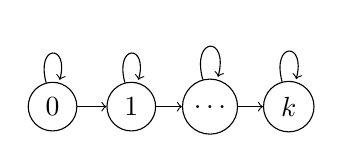
\begin{tikzpicture}[main/.style = {draw, circle}] 
    \node[main] (0) {$0$}; 
    \node[main] (1) [right of=0] {$1$};
    \node[main] (2) [right of=1] {$\hdots$}; 
    \node[main] (3) [right of=2] {$k$};
    
    \draw[->] (0) -- (1);
    \draw[->] (1) -- (2);
    \draw[->] (2) -- (3);
    \draw (0) edge [loop above] node {} (0);
    \draw (1) edge [loop above] node {} (1);
    \draw (2) edge [loop above] node {} (2);
    \draw (3) edge [loop above] node {} (3);
 \end{tikzpicture} \\
         \textbf{Graph 1: Binary String with k Zeros.}
      \item Construct a graph with 7 verteces representing all the combinations 
         that the last two characters can take on. 
         The * character represents a missing character 
         if the string length is less than 2.

         Each edge represents changing the string by adding a zero or one
         (The right symbol of the successor vertex of the edge is the added symbol).
         Note that $00$ and $11$ do not have self-loops 
         to prevent three characters in a row.
         The length of a walk beginning at ** 
         is equal to the length of the associated string

         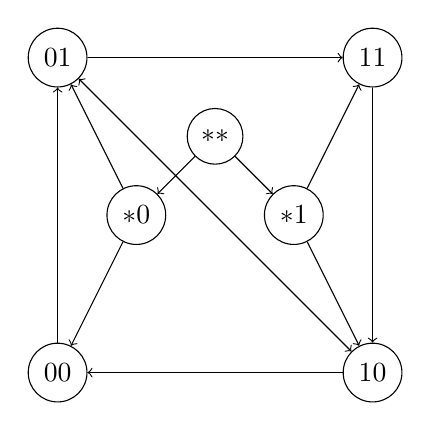
\begin{tikzpicture}[main/.style = {draw, circle}]
   \node[main] (**) at (0, 1) {$**$};
   \node[main] (*0) at (-1, 0) {$*0$};
   \node[main] (00) at (-2, -2) {$00$};
   \node[main] (01) at (-2, 2) {$01$};
   \node[main] (*1) at (1, 0) {$*1$};
   \node[main] (10) at (2, -2) {$10$};
   \node[main] (11) at (2, 2) {$11$};

   \draw[->] (**) -- (*1);
   \draw[->] (**) -- (*0);
   \draw[->] (*0) -- (00);
   \draw[->] (*0) -- (01);
   \draw[->] (*1) -- (10);
   \draw[->] (*1) -- (11);

   \draw[->] (00) -- (01);
   \draw[->] (11) -- (10);

   \draw[->] (01) -- (11);
   \draw[->] (10) -- (00);
   \draw[<->] (10) -- (01);
\end{tikzpicture} \\
         \textbf{Graph 2: Binary String Without Three Symbols in a Row.}
   \end{enumerate}
   \newpage 
\section{Painting Tables}
   \begin{enumerate}
      \item 
         Let $\alpha(S)$ be the set of ways to paint tables red,
         let $\beta(S)$ be the set of ways to paint tables blue,
         and let $\gamma(S)$ be the set of ways to paint tables green.
         Since $|\alpha(S)| = 1$ when $|S|$ is odd and
         $|\alpha(S)| = 0$ when $|S|$ is even,
         the exponential generating function for $\alpha$ is 
         \[
            E_\alpha(x) 
            = \sum_{n \geq 0} \frac{x^{2n+1}}{(2n+1)!}
            = \frac{e^x - e^{-x}}{2}.
         \]
         Similarly for $\beta$,
         \[
            E_\beta(x) 
            = \sum_{n \geq 0} \frac{x^{2n}}{(2n)!}
            = \frac{e^x + e^{-x}}{2}.
         \]
         We have that $E_\gamma(x) = e^x$ since $|\gamma(S)| = 1$.
         The exponential generating function for painting tables is
         \begin{align*}
            E_{\alpha\cdot\beta\cdot\gamma}(x) 
            &= \frac{1}{4}e^x(e^x - e^{-x})(e^x + e^{-x}) \\
            &= \frac{1}{4}(e^{3x}-e^{-x}) \\
            &= \frac{1}{4}\left(\sum_{n\geq 0} \frac{(3x)^n}{n!} 
               + \sum_{n\geq 0} \frac{(-x)^n}{n!}\right).
         \end{align*}
         Therefore, the number of ways to paint $n$ tables 
         according to the listed rules is $\frac{1}{4}(3^n + (-1)^n)$.
      \item Let $\delta(S)$ be the set of ways to paint tables white or yellow.
         Since $|\delta(S)| = 2^{|S|}$ when $|S|$ is even and
         $|\delta(S)| = 0$ when $|S|$ is odd,
         the exponential generating function for $\delta$ is 
         \[
            E_\delta(x) 
            = \sum_{n \geq 0} \frac{(2x)^{2n}}{(2n)!}
            = \frac{e^{2x} - e^{-2x}}{2}.
         \].
         The new exponential generating function for painting tables is 
         \begin{align*}
            E_{\alpha\cdot\beta\cdot\gamma\cdot\delta}(x) 
            &= \frac{1}{8}(e^{3x}-e^{-x})(e^{2x} - e^{-2x}) \\
            &= \frac{1}{8}(e^{5x}-2e^x+e^{-3x}).
         \end{align*}
         The number of ways to paint $n$ tables is now 
         $\frac{1}{8}(5^n+(-3)^n-2)$.
   \end{enumerate}
   \newpage
\section{EGF of set partitions and even blocks.}
   \begin{enumerate}
      \item Let $\alpha(S)$ be the set of ways to have a set partition 
         with a single even block.
         Note that $\alpha(\emptyset) = \emptyset$.
         The EGF of $\alpha$ is 
         \[
            E_\alpha(x)
            = \sum_{n \geq 1} \frac{x^{2n}}{(2n)!}
            = \frac{e^x + e^{-x}}{2} - 1
            = \frac{e^x + e^{-x}-2}{2}.
         \]
         We have that
         \[
            B_k(x)
            = E_{\alpha^k}(x)
            = \left(\frac{e^x + e^{-x}-2}{2}\right)^k.
         \]
      \item If there is no restriction on the number of blocks, then
         \[
            B(x) 
            = E_{e^\alpha}(x)
            = \exp\left(\frac{e^x + e^{-x}-2}{2}\right).
         \]
   \end{enumerate}
   \newpage 
\section{Idempotent Functions }
   The idempotent function $f:[n] \to [n]$ can be encoded as a directed graph 
   with vertices $[n]$ and an edge $i \to j$ if $f(i) = j$.
   If there is an edge $i \to j$ then there must also be a self-loop $j \to j$.
   Let $\alpha(S)$ be the set of ways to have a 
   connected graph with only one self-loop.
   Since there are $|S|$ possible choices for the vertex with the self-loop,
   \[
      E_\alpha(x)
      = \sum_{n \geq 1} n\frac{x^{n}}{(n)!}
      = x\sum_{n \geq 1} \frac{x^{n-1}}{(n-1)!}
      = xe^x.
   \]
   Thus, 
   \[
      A(x) 
      = E_{e^\alpha}(x)
      = \exp(xe^x).
   \]
\end{document}